\documentclass[10pt,handout,english]{beamer}
\usepackage[compatibility=false]{caption}
\usepackage[english]{babel}
\usepackage[backend=biber,style=numeric-comp,sorting=none]{biblatex}
\usepackage{amsmath}
\usepackage{amssymb}
\usepackage{graphicx,caption,copyrightbox}
\usepackage{hyperref}
\usepackage{color}
\usepackage{subcaption}
\usetheme{Berlin}
\beamertemplatenavigationsymbolsempty
\captionsetup{justification=centering, labelfont=sc, labelsep=endash}

\title[Joke Recommendation]{Intelligent Data Analysis II -\\Joke Recommendation}
\subtitle{Recommender System}
\author[Baptiste O'Jeanson]{Baptiste~O'Jeanson}
\institute[Potsdam University]{Institute of Computer Science}
\date{}
\subject{Computer Science}

\AtBeginSubsection[]
{
  \begin{frame}
    \frametitle{Table of Contents}
    \tableofcontents[currentsection, currentsubsection, subsubsectionstyle=hide]
  \end{frame}
}

\expandafter\def\expandafter\insertshorttitle\expandafter{%
  \insertshorttitle\hfill%
  \insertframenumber\,/\,\inserttotalframenumber}

\begin{document}

	\maketitle

	\begin{frame}
	\frametitle{Table of Contents}
	\tableofcontents[currentsection, sectionstyle=show, subsectionstyle=show, subsubsectionstyle=hide]
	\end{frame}

	\section{Introduction}
		%\subsection{What is a recommender system ?}
		%	\begin{frame}
		%	\frametitle{What is a recommender system ?}
		%		\begin{itemize}
		%			\item \textbf{Jeffrey M. O'Brien said in ``The race to create a smart Google''\footnote{\url{http://archive.fortune.com/magazines/fortune/fortune_archive/2006/11/27/8394347/index.htm}} :}\\~\\
		%			``The Web, they say, is leaving the era of \textcolor{blue}{search} and entering one of \textcolor{blue}{discovery}. What's the difference? Search is what you do when you're looking for something. Discovery is when something wonderful that you didn't know existed, or didn't know how to ask for, finds you.''
		%		\end{itemize}

		%	\end{frame}

		\subsection{The value of recommendation}
			\begin{frame}
				\frametitle{The value of recommendation}
				\begin{columns}[c]
					\column{.5\textwidth}
						\begin{itemize}
							\item Netflix : 75\% of the movies watched are recommended\\~\\~\\
							\item Spotify :  71\% of Discover Weekly\footnotemark[2] listeners saved at least one track to their own playlists\\~\\~\\
							\item Amazon: 35\% sales from recommendations
						\end{itemize}
					\column{.5\textwidth}
						\begin{figure}[h!]
				        	\centering
			            	
\includegraphics[width=0.4\textwidth]{netflix.png}
			                \label{fig:netflix}
			            \end{figure}
			            \begin{figure}[h!]
				            \begin{subfigure}[b]{0.4\textwidth}
				            	\centering
				                
\includegraphics[width=\textwidth]{pandora.jpg}
				            \end{subfigure}
				            \begin{subfigure}[b]{0.4\textwidth}
				            	\centering
				                
\includegraphics[width=\textwidth]{spotify.png}
				            \end{subfigure}
				        \end{figure}
						\begin{figure}[h!]
			            	\centering
			                
\includegraphics[width=0.6\textwidth]{amazon.jpg}
				        \end{figure}
				\end{columns}
				\footnotetext[2]{Discover Weekly brings you two hours of custom-made music recommendations, tailored specifically to you and delivered as a unique Spotify playlist.}
			\end{frame}

		\subsection{The ``Recommender problem''}
			\begin{frame}
			\frametitle{The ``Recommender problem''}
				\begin{itemize}
					\item Estimate a \textcolor{blue}{utility function} that \textcolor{blue}{automatically predicts} how a user will \textcolor{blue}{like} an item.
					\item Based on:
						\begin{itemize}
							\item Past behavior
							\item Relations to other users
							\item Item similarity
							\item Context
							\item ...
						\end{itemize}
					\item Don't recommend items the user already knows or would have found anyway.
					\item Expand the user's taste into neighboring areas (improve the obvious).
				\end{itemize}

			\end{frame}

			\begin{frame}
			\frametitle{Problem Setting}
				\begin{columns}[c]
					\column{.4\textwidth}
						{\small \begin{itemize}
							\item Users $U = \{1, ... , m\}$
							\item Items $X = \{1, ... , m^\prime\}$
							\item Ratings $Y = \{(u_1, x_1, y_1)\ldots, (u_n, x_n, y_n)\}$
							\item Utility function \textbf{f} measure the usefulness of item \textbf{x} to user \textbf{u} : \boldmath{$f : U~x~X \rightarrow R$}.
							\item For each user \textbf{$u\in U$}, we want to choose items \textbf{$x \in X$} that maximize \textbf{$f$}.\\
							\end{itemize}
						}
					\column{.6\textwidth}
						\begin{figure}[h!]
			            	\centering
			                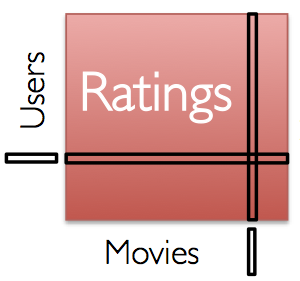
\includegraphics[width=\textwidth]{matrix_rating.png}
				        \end{figure}
				\end{columns}
			\end{frame}

		\subsection{Two-step process}
			\begin{frame}
			\frametitle{Two-step process}
				\begin{figure}[h!]
	            	\centering
	                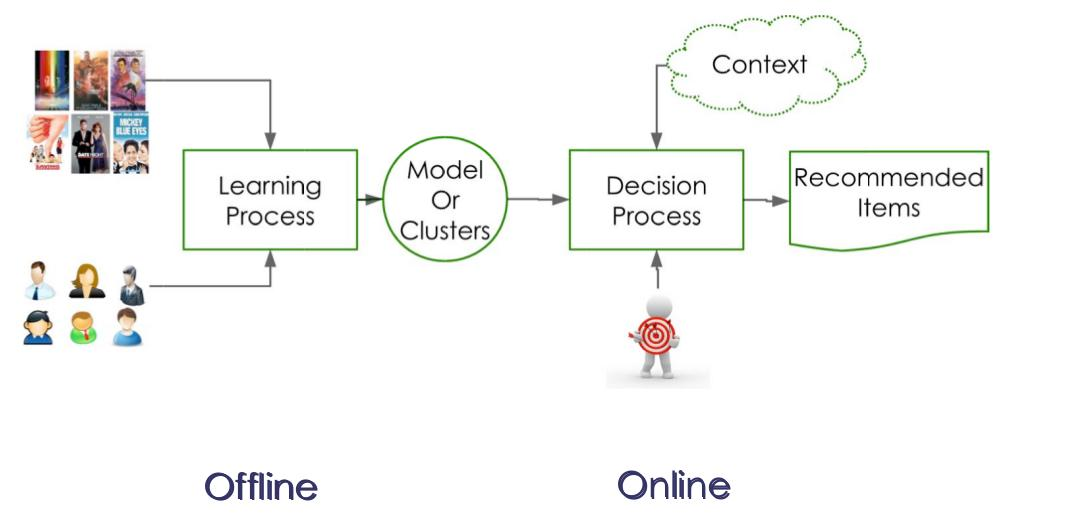
\includegraphics[width=\textwidth]{two_step_process.jpg}
		        \end{figure}

			\end{frame}

	\section{Approaches to Recommendation}
		\subsection{Overview}
			\begin{frame}
			\frametitle{Overview}
				\begin{itemize}
					\item Collaborative Filtering : Recommend items based only on the users past behavior
						\begin{itemize}
							\item User-based
							\item Item-based
						\end{itemize}
					\item Content-based : Recommend based on item features
					\item Novel methods :
						\begin{itemize}
							\item Context-aware Recommendations
							\item Deep Learning
						\end{itemize}
					\item Hybrid approaches : Combine any of the above
				\end{itemize}

		\end{frame}

		\subsection{Collaborative Filtering}
			\subsubsection{Principle}
			\begin{frame}
			\frametitle{Principle}
				\begin{block}{Idea of collaborative filtering}
					Determine the users' preferences from \textbf{historical usage data}.
				\end{block}~\\
				For example, if two users listen to largely the same set of songs, their tastes are probably similar. Inversely, if two songs are listened by the same group of users, they probably sound similar.\\~\\~\\

				\textbf{Pure} collaborative filtering : no use of any kind of information about the items : content-agnostic.

			\end{frame}

			\subsubsection{Item-based CF with Nearest Neighbor}
			\begin{frame}
			\frametitle{Item-based CF with Nearest Neighbor}
				\begin{block}{Idea of Item-based CF with Nearest Neighbor}
					For a target item i (one the user did not rate) :
					\begin{enumerate}
						\item Compute how similar the set of items already rated (by the target user) are to the target item i
						\item Select k most ``similar'' items $\{i_1, i_2, \ldots, i_k\}$
						\item The prediction is computed by taking a weighted average of the target user's ratings on these similar items.
					\end{enumerate}
				\end{block}~\\

				For step 2, use Nearest Neighbor with :
				\begin{itemize}
					\item the Pearson correlation
					\item or the cosine metrics or the adjusted cosine similarity.\\~\\
				\end{itemize}
				\textcolor{blue}{In the lecture, we focused on user).}


			\end{frame}

			\begin{frame}
			\frametitle{Item-based CF with Nearest Neighbor : Discussion}
				\begin{itemize}
					\item Bottleneck : similarity computation
					\item Scalability : Nearest Neighbor's computation grows with both the number of users and items.
					\item Isolate the neighborhood generation and predication steps (``off-line'' similarity computation, ``on-line'' prediction generation)
					\item Item-based CF : enables the pre-computing of the item-item similarity (the prediction process : only a table lookup for the similarity values and computation of the weighted sum).\\~\\
				\end{itemize}
				User-based CF with Nearest Neighbor : pre-computing user neighborhood can lead to poor predictions ($\rightarrow$ latent feature).

			\end{frame}

			\subsubsection{User-based CF with Matrix Factorization}
			\begin{frame}
			\frametitle{User-based CF with Matrix Factorization}
				\begin{block}{Idea of User-based CF with Matrix Factorization}
					Learn feature that represent the user preferences by modeling each user/item as a vector of factors :
						$Y = \Psi \Theta$
				\end{block}
				\begin{figure}[h!]
	            	\centering
	                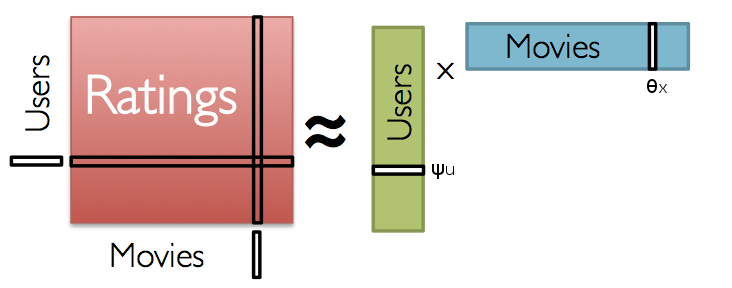
\includegraphics[width=0.7\textwidth]{matrix_factorization.png}
		        \end{figure}
		        Use Singular Value Decomposition (SVD) to factorize the matrix.

			\end{frame}

			\begin{frame}
			\frametitle{User-based CF with Matrix Factorization : Discussion}
				\begin{itemize}
					\item SVD was one of the algorithm used by the winners of Netflix Competition
					\item Limitations : Not adaptable as users add ratings
				\end{itemize}

			\end{frame}

			\subsubsection{Discussion}
			\begin{frame}
			\frametitle{Discussion}
				\begin{itemize}
					\item \textbf{Advantages :}
						\begin{itemize}
							\item Requires minimal knowledge engineering efforts
							\item Produces good-enough results in most cases
						\end{itemize}
					\item \textbf{Disadvantages :}
						\begin{itemize}
							\item Cold Start problem : Requires a large number of user feedback data ratings to bootstrap.
							\item Long Tail problem : Reliance on usage data induces that popular items are much easier recommended than unpopular items (there is more usage data available for them)
							\item Assumes that prior behavior determines current behavior (no ``contextual'' knowledge)
						\end{itemize}
				\end{itemize}

			\end{frame}

		\subsection{Content-based Recommendation}
			\subsubsection{Principle}
			\begin{frame}
			\frametitle{Principle}
				\begin{block}{Idea of Content-based Recommendation}
					The recommendations are based on information on the content of items rather than on other users' opinions/interactions.
				\end{block}

				Pure content-based recommendation for a user based only on analyzing the content of items rated in the past by the user :
				\begin{itemize}
					\item Can be explicit attributes or characteristics of the item.
					\item Can be textual content (use NLP techniques)
					\item Can be extracted from the signal (audio, image) itself (with Fourier transformation)
				\end{itemize}

			\end{frame}

			\subsubsection{Discussion}
			\begin{frame}
			\frametitle{Discussion}
				\begin{itemize}
					\item \textbf{Advantages :}
						\begin{itemize}
							\item No need for data on other users (No Cold Start or sparsity problems)
							\item Able to recommend to users with unique tastes
							\item Able to recommend new and unpopular items (No Long Tail problem)
							\item Can provide explanations by listing content-features that caused an item to be recommended.
						\end{itemize}
					\item \textbf{Disadvantages :}
						\begin{itemize}
							\item Requires content that can be encoded as meaningful features and carries users' tastes
							\item Some items have no easy feature extraction methods (movies, musics)
							\item Easy to overfit (e.g. for a user with few data points)
						\end{itemize}
				\end{itemize}
			\end{frame}


		\subsection{Novel methods}
			\subsubsection{Context-aware Recommendations}
			\begin{frame}
			\frametitle{Context-aware Recommendations}
				\begin{columns}[c]
					\column{.4\textwidth}
						\begin{figure}[h!]
			    		    \centering
			                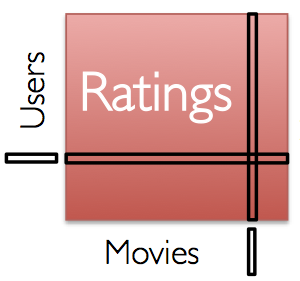
\includegraphics[width=0.7\textwidth]{matrix_rating.png}
		             	\end{figure}
		            \column{.6\textwidth}
		            	\begin{figure}[h!]
			            	\centering
			                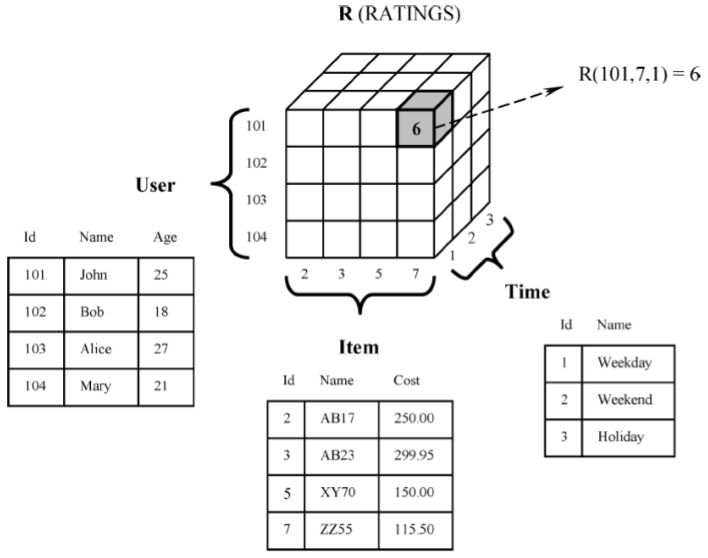
\includegraphics[width=0.7\textwidth]{context_recommendation.png}
			            \end{figure}
			        \end{columns}
			    Most popular approaches are Tensor Factorization and Factorization Machines.\\ See \url{http://fr.slideshare.net/SessionsEvents/steffen-rendle-research-scientist-google-at-mlconf-sf}

			\end{frame}

			\subsubsection{Deep Learning for Collaborative Filtering}
			\begin{frame}
			\frametitle{Deep Learning for Collaborative Filtering}
				\begin{itemize}
					\item Spotify : See \url{http://benanne.github.io/2014/08/05/spotify-cnns.html}
					\item Netflix : See \url{http://techblog.netflix.com/2014/02/distributed-neural-networks-with-gpus.html}
				\end{itemize}
            	\begin{figure}[h!]
	            	\centering
	                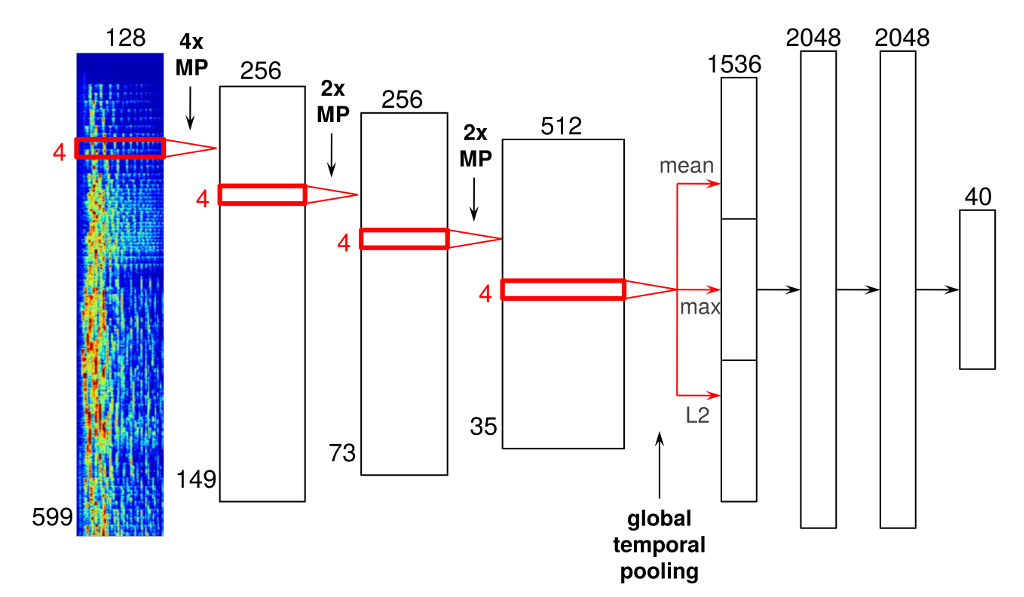
\includegraphics[width=0.7\textwidth]{spotify_convnet.png}
	            \end{figure}
			\end{frame}

	\section{Joke Recommendation}
		\subsection{The Jester dataset}
			\begin{frame}
			\frametitle{The Jester dataset}
			\begin{itemize}
				\item Very diverse set of jokes that would appeal to specific audiences (Specific countries, Specific age groups, $\ldots$)
				\item No jokes that would appeal to all audience (user-specific nature of a recommender system exploited)
				\item The rating are in the interval $[-10, +10]$
			\end{itemize}
			This dataset were gathered applying the ``Eigentaste'' Algorithm\\~\\
			Two files : the text of the jokes and a matrix including 150 jokes rated by 59,132 users

			\end{frame}

		\subsection{The ``gauge set''}
			\begin{frame}
			\frametitle{The ``gauge set''}
				\begin{itemize}
					\item Set of items with the highest variance in the system : allows quick identification of other users with similar preferences.
					\item All users have to rate the gauge set of items :
						\begin{itemize}
							\item No cold start problem for new users.
							\item The gauge set ratings matrix is dense, which allows to application PCA
						\end{itemize}
				\end{itemize}

			\end{frame}

		\subsection{Eigentaste 5.0 (Algorithm)}
			\begin{frame}
			\frametitle{Eigentaste 5.0 (Algorithm) 1/3}
				Offline process :
				\begin{itemize}
					\item Cluster the item space into groups of similar items across all users' rating with k-means and Pearson correlation as distance metric
					\item Cluster users into groups with similar taste and aggregating their ratings : help predicting how a new user would rate the items :
						\begin{enumerate}
							\item PCA on the ratings matrix of the gauge set
							\item Each user is projected onto the resultant eigenplane (2 first eigenvalues)
							\item High concentration of users around the origin : a median-based algorithm (recursive rectangular clustering) applied on the PCA space to divide users into clusters
						\end{enumerate}
				\end{itemize}

			\end{frame}

			\begin{frame}
			\frametitle{Eigentaste 5.0 (Algorithm) 2/3}
				Online process for a new user :
				\begin{enumerate}
					\item Rating the gauge set and the ``seed set'' (set of jokes with the fewest number of ratings)
					\item The user is projected into the principal components space
					\item The user falls into one of the clusters defined offline
					\item The user rate the ``recommendation set'' : the system predict the user’s rating for every joke and sorts them.\\~\\
				\end{enumerate}

			\end{frame}

			\begin{frame}
			\frametitle{Eigentaste 5.0 (Algorithm) 3/3}
				Prediction process :
				\begin{itemize}
					\item For each user u we maintain a vector $\overrightarrow{a_u}$ of a moving average of u's ratings of the items in each item cluster.
					\item Initialized with his ratings of items from the common set.
					\item $\overrightarrow{a_u}[c]$ corresponds to user u's average rating of the last n items in item cluster c\\~\\
				\end{itemize}
				\begin{tabular}{|l|c|r|}
					\hline
					Item Cluster & User u's last 5 ratings & Average \\
					\hline
					1 & 4.2, 5.3, 3.8, 2.1, 2.7 & 3.62 \\
					2 & 7.2, 6.5, 5.9, 0.8, -1.2 & \textbf{3.84} \\
					3 & 1.9, -2.4, 3.8, 2.1, 0.5 & 1.18 \\
					\hline
				\end{tabular}
			\end{frame}


			\begin{frame}
			\frametitle{Eigentaste 5.0 : Discussion}
				\begin{itemize}
					\item Advantages :
						Run in constant online time
					\item Disadvantages :
						Impossible to truly compare how a user would react to different item recommendation orders, as the first test would greatly bias the second.
				\end{itemize}
				\begin{figure}[h!]
	            	\centering
	                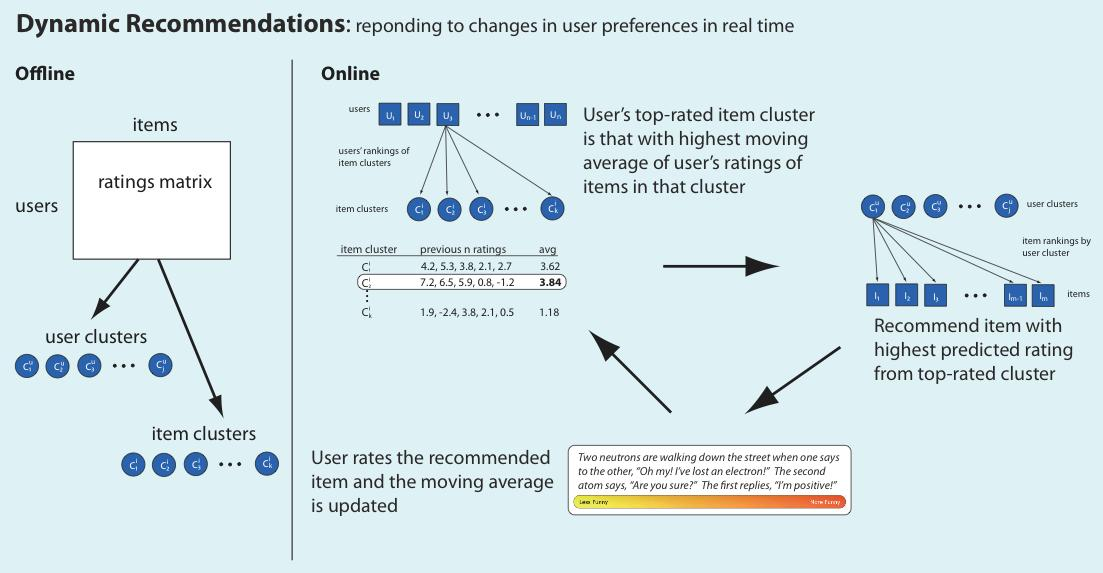
\includegraphics[width=0.9\textwidth]{eigentaste.jpg}
	            \end{figure}

			\end{frame}

		\subsection{My work}
			\begin{frame}
			\frametitle{My work 1/3}
				\begin{block}{Idea}
					Use Item-based Collaborating Filtering approach with content-base one :\\
					Add some content-based features extracted from the jokes (text).
				\end{block}
				Methodology :
				\begin{enumerate}
					\item Extract the textual jokes from the HTML file and normalize them :
					\begin{enumerate}
						\item Tokenization
						\item Compute Part-of-Speech Tagging
						\item Use POS Tagging to improve Lemmatization
						\item Remove stopwords and puntuation
					\end{enumerate}
					\item Transform the normalized jokes in the bag-of-words representation
					\item Apply Latent Dirichlet Allocation on the bag-of-words
					\item Compute Cosine Similarity on the ``joke/topic'' matrix
				\end{enumerate}

			\end{frame}

			\begin{frame}
			\frametitle{My work 2/3}
				For a target joke i (one the user did not rate) :
				\begin{enumerate}
					\item Compute how similar the set of jokes already rated (by the target user) are to the target joke i
					\item Select k most ``similar'' jokes $\{i_1, i_2, \ldots, i_k\}$
					\item The prediction is computed by taking a weighted average of the target user's ratings on these similar jokes.\\~\\
				\end{enumerate}

				For step 2, use Nearest Neighbor with the cosine metrics.

			\end{frame}


			\begin{frame}
			\frametitle{My work 3/3}
				Model the rating $y_{ij}$ that user i likes joke j as the user's affinity to the topics contained in all jokes :\\
				$y_{ij} = \psi_{i} * \theta{j} + \sum_{k} s_{ik}\bar{z}_{jk}$\\~\\
				$s_{ik}$ : User i's affinity to topic k\\~\\
				$P_r(joke_j~has~topic_k)$ : probability that the joke j contains the LDA topic k / proportion of the topic k in joke j

			\end{frame}

	\section{Conclusion}
		\begin{frame}
		\frametitle{Conclusion}
			\begin{itemize}
				\item For content-based approach, very difficult to extract informative feature
				\item The Dataset was built using the Eigentaste application
				\item Difficult to automate the 2-step process
			\end{itemize}

		\end{frame}


	\appendix
	\newcounter{finalframe}
	\setcounter{finalframe}{\value{framenumber}}
	% Backup frames
	\setcounter{framenumber}{\value{finalframe}}

\end{document}